\documentclass[conference]{IEEEtran}
\IEEEoverridecommandlockouts
% The preceding line is only needed to identify funding in the first footnote. If that is unneeded, please comment it out.
\usepackage{cite}
\usepackage{placeins}
\usepackage{amsmath,amssymb,amsfonts}
\usepackage{algorithmic}
\usepackage{graphicx}
\usepackage{textcomp}
\usepackage{xcolor}
\def\BibTeX{{\rm B\kern-.05em{\sc i\kern-.025em b}\kern-.08em
    T\kern-.1667em\lower.7ex\hbox{E}\kern-.125emX}}
\begin{document}

\title{Assessment and Evaluation of an Unsupervised Machine Learning Model for Automotive and Industrial NVH Applications\\
{\footnotesize \textsuperscript}
%\thanks{Identify applicable funding agency here. If none, delete this.}
}

\author{\IEEEauthorblockN{ Abdul Haq Azeem Paracha}
\IEEEauthorblockA{\textit{Institute Of Media Technology} \\
\textit{Technische Universität Ilmenau}\\
Ilmenau, Germany \\
abdulhaq.ah@gmail.com}
\and
\IEEEauthorblockN{ Johannes Blickensdorff}
\IEEEauthorblockA{\textit{dept. name of organization (of Aff.)} \\
\textit{Schaeffler Gruppe}\\
City, Germany \\
johannes.blickensdorff@schaeffler.com}
\and
\IEEEauthorblockN{Dr. David Scott Johnson}
\IEEEauthorblockA{\textit{dept. name of organization (of Aff.)} \\
\textit{name of organization (of Aff.)}\\
City, Germany \\
email address or ORCID}


}

\maketitle

\begin{abstract}
Current NVH analysing techniques involve an interdisciplinary knowledge of structural dynamics, signal processing, technical- and psycho-acoustics but most notably they require an experienced professional to analyse and assess the ever-expanding amount of industrial acquired NVH data.
Recent advances in machine learning (ML) have shown the possibilities of inference on feature representations of input data without human intervention, which has helped experts to focus on actual solutions and reduce manual efforts for pre-processing and classification significantly. \cite{b1}
We challenged an unsupervised deep neural network model (DNN) based on autoencoders (AE) to detect anomalies and semantic relations in different types of industrial NVH data and compared findings with an analytical state of the art approach. \cite{b2}


\end{abstract}

\begin{IEEEkeywords}
component, formatting, style, styling, insert
\end{IEEEkeywords}

\section{Introduction}
ML algorithms provide key methods to improve the ability of machines to learn, the main idea behind ML is inductive inference, through which specific statistical phenomena is generalized \cite{b4}.The rapid change in the industry like the emergence of electric vehicle (EV) and increasing in the data has posed a serious challenge for NVH engineers. The classical approach for NVH data analysis requires assessment of individual channels with many signal processing techniques, in depth analysis is required to confirm properties with respect to design and simulation.
\subsection{Abbreviation and Acronyms}\label{AA}
Noise Vibration Harshness (NVH), Machine Learning (ML), deep neural network (DNN), Short Time Fourier Transform (STFT), Measuring Point (MP), Device Under Test (DUT), End of Line (EoL), Electric Drive Unit (EDU), Multilayer Perceptron (MLP), Autoencoder (AE), Area Under Curve (AUC), Mean Square Error (MSE), Mean Absolute Error (MAE), Rectified Linear Unit (ReLU). 

\section{Related Work}
The complexity of acoustic parameters is reduced manually to achieve a set of basic criteria to define metrics \cite{b3}. In comparison to traditional handcrafted features extraction and analysis the DNN provides an alternative approach of feature learning which has shown significant success in image and speech recognition applications \cite{b1}. The benchmarking of accuracy for this research is classical NVH analysis by human experts. The ML algorithm performance is greatly dependent on the choice of data features \cite{b1}.Therefore this research is focused on comparison of STFT and order features.    



\section{Dataset}
The industrial NVH datasets generally include either airborne noise or structure borne noise data. The common transducers used for data collection are microphone and accelerometers. The sampling rate is often from mid to high range. NVH datasets have multichannel data, which include data from multiple MP, with each MP having three axis (x, y, z) data. It also includes reference data like temperature, torque and rotational speed. The NVH R\&D dataset has a small number of DUT while EoL has a large number of DUT’s. The dataset used in this research is the EoL dataset. The industrial EoL data used represents end of line data of EDU or gears. The dataset consists of 77 samples, 70 samples identified as normal and 7 samples as fault through classical fault diagnosis by an expert. There are a total 6 channels in each sample with 2 reference channels. The data is collected at two MP, one at MP is at test bench and has three axis (x, y, z) data, while the other MP is on the DUT with a single tactile sensor. The reference channels are torque and rotational speed.  



\section{Methodology}
The methodology for evaluation of MLP AE on the EoL dataset consists of three steps: pre-processing, training and analysis. The dataset is divided into three subsets, training,  validation, and test data. The most important step in the evaluation of AE is to train the model only on the normal data. Therefore it is ensured to keep the training and validation data separate from the fault data. The training and validation data includes all the normal samples while the test data includes fault data. The loss or cost function used in AE is MSE, the error is minimized between input and output to reconstruct the data sample. The MAE is calculated between the original input data and predicted output data to find reconstruction error. In the analysis, part reconstruction error distribution of all the samples is visualized. The performance metric used is the AUC of precision and recall curve. Furthermore, based on the distribution of reconstruction error, the overlap of normal and fault samples is separated by a threshold value. The threshold is defined by the intersection point of precision and recall vs threshold curve. Finally, the confusion matrix is used to visualize the true positives.     
\section{Tools}
The main tool used for machine learning application is Python and its open-source libraries. The model is implemented in Tensorflow, through Keras API. The STFT features are extracted though Python piplines, while order features are extracted through integration of Matlab and Python. The dataset industrial file formats are converted through IMC Famos.   

\section{Experimental Setup}

One data channel is used along with a rotational speed channel in the preprocessing step. The Order and STFT features are extracted. The procedure of anomaly detection demands the test data include both normal samples and fault samples. Therefore 63 out of 70 normal samples are used for training and validation of the model. The 7 normal samples and 7 fault samples are used in the test subset. After feature extraction, all the data is scaled through min-max scaling. The model used for training uses ReLU as an activation function, it has 10 layers. The first layer of the encoder starts with 256 neural units and progressively decreases to 16 units in the latent space. The decoder starts with 16 units and increases to 256 units in the last layer. The optimization algorithm used is Adam.

\section{Results and Discussion}
There were two experiments conducted with the same model parameters, experiment A and experiment B. The experiment A is using STFT features while experiment B is using Order features. The training and validation loss for both experiments is 0.04. The threshold of experiment A according to precision and recall vs threshold curve is 0.169 as shown in figure \ref{fig:threshold_expa}.


\begin{figure}[htbp]
\centerline{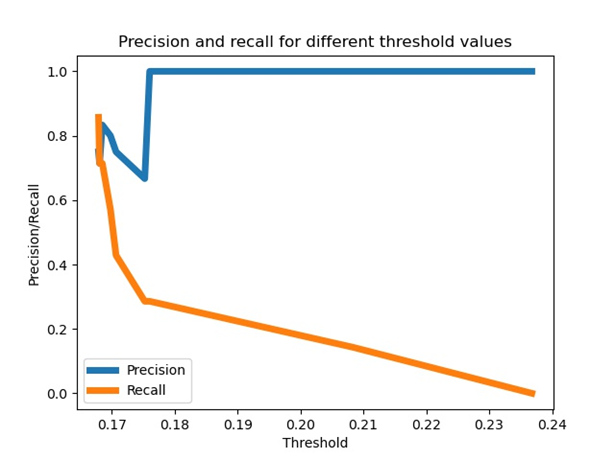
\includegraphics[scale=0.5]{stft_threshold.png}}
\caption{Precision and recall curves with respect to threshold while training with STFT features, experiment A}
\label{fig:threshold_expa}
\end{figure}

 The threshold for experiment B is 0.166 as shown in figure \ref{fig:threshold_expb}.

\begin{figure}[htbp]
\centerline{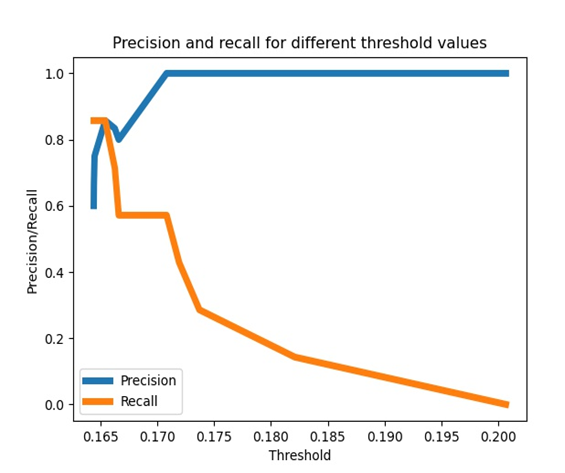
\includegraphics[scale=0.5]{order_threshold.png}}
\caption{Precision and recall curves with respect to threshold while training with order features, experiment B}
\label{fig:threshold_expb}
\end{figure}

The AUC of precision-recall curve for experiment A is 0.828 while for experiment B is 0.878 as shown in figure \ref{fig:auc_expa_expb}.  

\begin{figure}[htbp]
\centerline{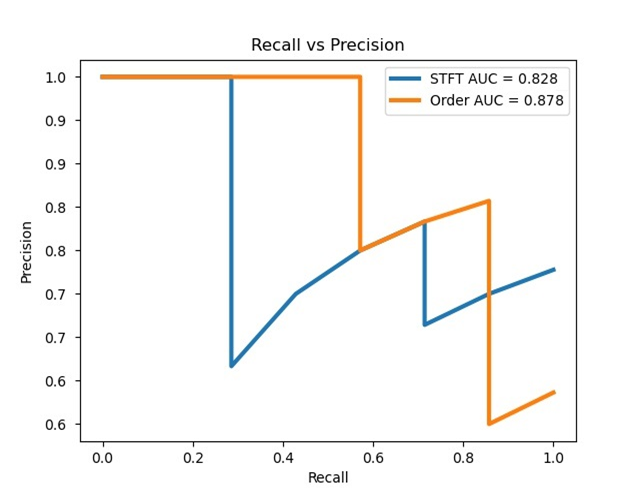
\includegraphics[scale=0.45]{auc.png}}
\caption{Performance if experiment A and B through AUC precision vs recall curve}
\label{fig:auc_expa_expb}
\end{figure}

A more detailed analysis of the experiment A can be seen in figure \ref{fig:conf_matrix_expa}. The true class shows the annotations identified by an NVH expert through classical analysis. The predicted class is the model output. The predicted faulty label indicate true positives.     

\begin{figure}[htbp]
\centerline{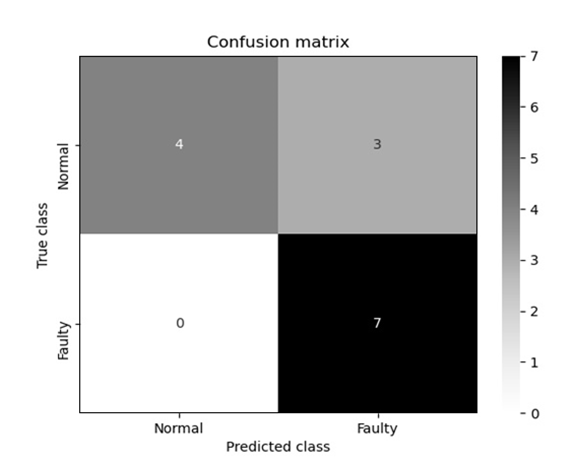
\includegraphics[scale=0.5]{conf_matrix_stft.png}}
\caption{Confusion matrix experiment A}
\label{fig:conf_matrix_expa}
\end{figure}

As shown in figure \ref{fig:conf_matrix_expb} all the 7 fault samples are correctly identified based on threshold in figure \ref{fig:threshold_expa}, but 3 normal samples are also wrongly categorized as faulty. In experiment B 7 out of 6 samples are correctly identified while 1 normal sample is identified as faulty and 1 faulty sample is identified as normal.    

\begin{figure}[htbp]
\centerline{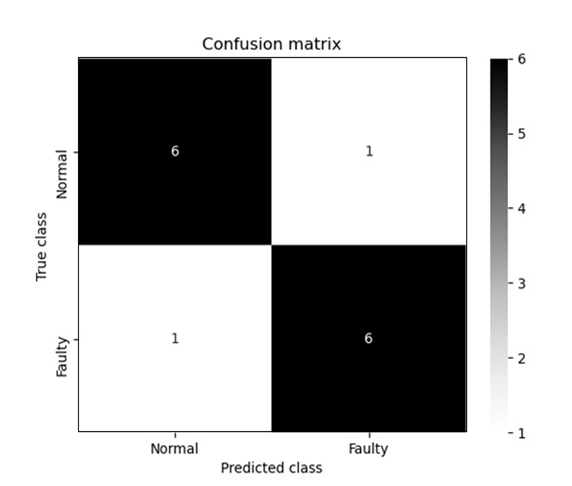
\includegraphics[scale=0.5]{conf_matrix_order.png}}
\caption{Confusion matrix experiment B}
\label{fig:conf_matrix_expb}
\end{figure}
\FloatBarrier
\section{Conclusion and Future Work}
The best comparative accuracy achieved is 0.878 in experiment b for order features. The classical approach requires in depth analysis of simulated, normal and failed data, with different signal processing techniques and many tools. AE only requires normal data with in depth analysis to find potentially faulty specimens. This data driven method and a good comparative accuracy to classical approach is promising and can help to reduce time consuming tasks of data examination of NVH engineers. The experiment results of this industrial NVH dataset are good but to achieve model inference more tests on new data will be required.   

\section*{Acknowledgment}

This research is conducted in collaboration of Schaeffler Gruppe and Fraunhofer IDMT. A special thanks to schaeffler Gruppe for providing industrial NVH dataset for this research.   


\begin{thebibliography}{00}
\bibitem{b1}Bengio, Yoshua et al. "Representation learning: A review and new perspectives". IEEE transactions on pattern analysis and machine intelligence 35. 8(2013): 1798–1828.


\bibitem{b2}Koizumi, Yuma et al. "Unsupervised detection of anomalous sound based on deep learning and the neyman–pearson lemma". IEEE/ACM Transactions on Audio, Speech, and Language Processing 27. 1(2018): 212–224.


\bibitem{b3}Knieper, Johannes et al. "Methoden für die akustische Analyse und Bewertung von E-Achs-Getrieben". deutsche gesellschaft für akustik. (2020).


\bibitem{b4}Rätsch, Gunnar. "A brief introduction into machine learning". Friedrich Miescher Laboratory of the Max Planck Society. (2004).


\end{thebibliography}

\end{document}
